\hypertarget{track__objects__server_8cpp}{}\section{src/track\+\_\+objects\+\_\+server.cpp File Reference}
\label{track__objects__server_8cpp}\index{src/track\+\_\+objects\+\_\+server.\+cpp@{src/track\+\_\+objects\+\_\+server.\+cpp}}


R\+OS Service node of object tracker.  


{\ttfamily \#include \char`\"{}ros/ros.\+h\char`\"{}}\\*
{\ttfamily \#include \char`\"{}laser\+\_\+scanner\+\_\+infoscreen/track\+Objects.\+h\char`\"{}}\\*
{\ttfamily \#include $<$visualization\+\_\+msgs/\+Marker.\+h$>$}\\*
{\ttfamily \#include $<$vector$>$}\\*
{\ttfamily \#include $<$cmath$>$}\\*
{\ttfamily \#include $<$utility$>$}\\*
{\ttfamily \#include $<$armadillo$>$}\\*
{\ttfamily \#include \char`\"{}laser\+\_\+objects.\+hpp\char`\"{}}\\*
Include dependency graph for track\+\_\+objects\+\_\+server.\+cpp\+:\nopagebreak
\begin{figure}[H]
\begin{center}
\leavevmode
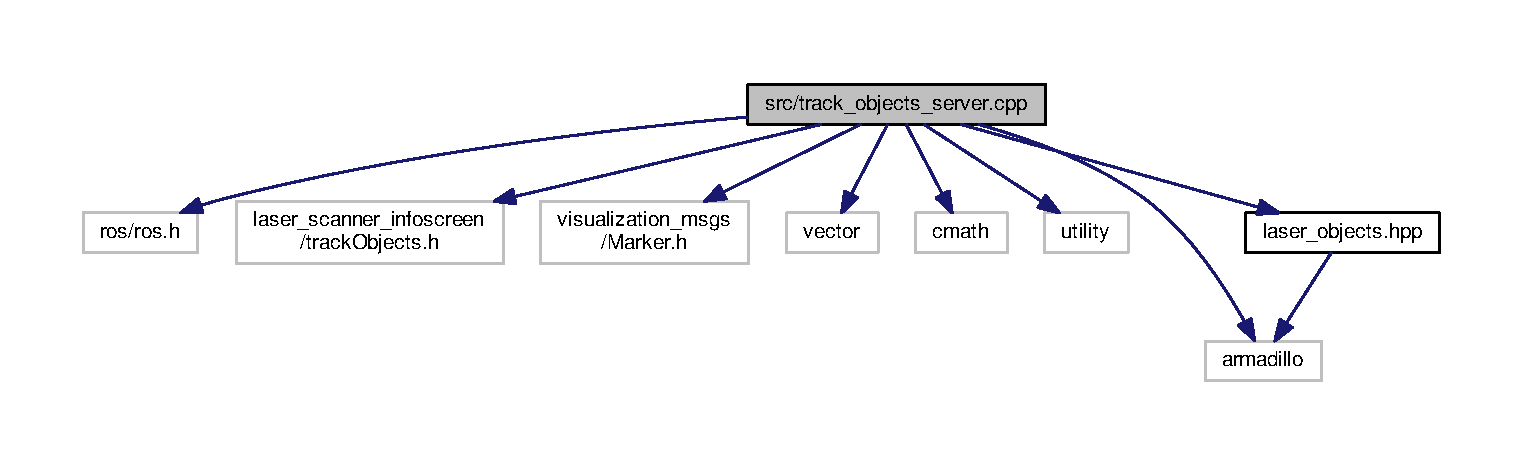
\includegraphics[width=350pt]{track__objects__server_8cpp__incl}
\end{center}
\end{figure}


\subsection{Detailed Description}
R\+OS Service node of object tracker. 

Handles low-\/level parsing Laser\+Scan message, and detecting and tracking objects. First culling is limiting wihtin 120deg cone to the front. Then points are broken into continuities of which between 0.\+4m and 0.\+7m long are passed to \hyperlink{classlaser__objects}{laser\+\_\+objects} for further processing.

\begin{DoxySeeAlso}{See also}
\hyperlink{track__objects__client_8cpp}{track\+\_\+objects\+\_\+client.\+cpp} 

\hyperlink{classlaser__objects}{laser\+\_\+objects} 
\end{DoxySeeAlso}
